\chapter{Protocol based on Spekkens contextuality}
\lhead{\emph{Protocol based on Spekkens contextuality}}
\label{sec:protocols}
We now generalize the self-testing result in \cite{Bharti2019}, which was discussed in Section \ref{sec:contselftesting}, to the framework of Spekkens contextuality. In particular, this will lift the usual restriction to noise-free projective measurements. Additional features will be discussed in Section \ref{sec:discussion}. The protocol we put forth assumes the approximate operational equivalence of some preparations, as well as an upper bound on the unknown system's information carrying capacity, much like the protocol in Section \ref{sec:contselftesting}.

Let $n\geq 5$ be an odd integer. The setting we consider is reminiscent of the ideal $n$-cycle reference experiment \ref{eqn:ncycleideal}. As such, we assume an experimenter to be able to freely choose between $n$ three-outcome measurements $\{M_i\}_{i=1}^n$, and label the outcomes $m_1$, $m_2$, $m_3$. We assume measurements to be chosen according to a uniform distribution and denote measurement events by  $m_k\thinspace\vert\thinspace M_i$, or $m_k,m_l\thinspace\vert\thinspace M_i,M_j$ for two sequential measurements. As shown in Figure \ref{fig:ncycleselftesting}, for an ideal device, the measurement events $m_1 \thinspace\vert\thinspace M_i$ correspond to the rank-one projectors $\vert u_i^{(n)}\rangle\langle u_i^{(n)}\vert$ defined by Equation \ref{eqn:ncycleideal}. Further, in the ideal case, the measurement events \begin{equation*}
m_3\thinspace\vert\thinspace M_i\equiv m_1\thinspace\vert\thinspace M_{i\oplus 1}\equiv\vert u_{i\oplus 1}^{(n)}\rangle\langle u_{i\oplus 1}^{(n)}\vert,
\end{equation*}and the events $m_2\thinspace\vert\thinspace M_i$ correspond to the projectors 
\begin{equation*}
m_2\,\vert\,M_i\equiv \mathbb{1}-\vert u_i^{(n)}\rangle\langle u_i^{(n)}\vert-\vert u_{i\oplus 1}^{(n)}\rangle\langle u_{i\oplus 1}^{(n)}\vert
\end{equation*} onto the pure qutrit state completing the orthogonal triad $\subset \mathbb{C}^3$. In Figure \ref{fig:ncycleselftesting}, the events $m_3\thinspace \vert\thinspace M_i$ and $m_1\thinspace\vert\thinspace M_{i\oplus 1}$ are ``non-overlapping", despite corresponding to the same ideal projectors, to highlight that we do not need to assume operational equivalence, contrary to the assumptions made in \cite{Kunjwal2019}.

\begin{figure}
	\begin{subfigure}[t]{0.45\textwidth}
    	\centering
    	\includegraphics[width=\textwidth]{images/mntsandpreps.png}
        \caption{}
	\end{subfigure}
	\hfill
    \begin{subfigure}[t]{0.45\textwidth}
    	\centering 
        \includegraphics[width=0.8\textwidth]{images/kcbsrefstates.png}
        \caption{}
    \end{subfigure}
    \caption[]{\textbf{(a):} Measurement events and retrospective preparations corresponding to a self-testing scenario consistent with the cycle length $n=5$. The experimenter can choose from five three-outcome measurements $M_i$, with outcomes $m_1,m_2,m_3$. In post-processing, the experimenter defines $2n$ preparations 

\begin{minipage}{\linewidth}
\vspace{0.2em}
     \begin{equation*}
        \{P_{m_k\vert M_i}\}_{k,i}\hspace{1em}\text{, for } k\in\{ 1,2\}\text{ and }i\in\{ 1,\dots,n\}.
     \end{equation*}    
\end{minipage}

\vspace*{0.7em} 
We additionally define $P_{m_3\vert M_i}\coloneqq P_{m_1\vert M_{i\oplus 1}}$. In the ideal case, the measurement events $\{m_k\vert M_i\}_{k\in\{1,2,3\}}$ correspond to rank-one projectors onto the orthogonal triad $\subset \mathbb{C}^3$ containing the cycle states $\vert u_i\rangle$ and $\vert u_{i\oplus 1}\rangle$. Furthermore, in the ideal case, the preparations $P_{m_k\vert M_i}$ are pure states that coincide with the vectors in this triad. The measurement events $m_3\vert M_i$ and $m_1\vert M_{i\oplus 1}$ are non-overlapping to illustrate that the self-testing protocol does not assume the operational equivalence of these, despite the fact that they correspond to the same rank-one projector onto $\vert u_{i\oplus 1}\rangle$ in the ideal case. \textbf{(b):} Juxtaposition with the cycle states belonging to the odd $n$-cycle scenario for $n=5$. Figure (a) can be seen as a top view of (b), with every black dot corresponding to a cycle state $\vert u_i\rangle$.
}
\label{fig:ncycleselftesting}
\end{figure}

Like in Section \ref{sec:contselftesting}, we assume i.i.d.\ rounds, i.e. the devices to operate in an identical manner for all rounds of the protocol, in particular independently of previous input-output cycles. This allows us to lift relative frequencies to probabilities. We will discuss all other assumptions in due time. The protocol consists of the following steps:
\begin{enumerate}
\item The experimenter prepares the system in a distinguished preparation $P_0$, by selecting the appropriate setting on the corresponding device.
\item The experimenter samples from a uniform distribution and selects two integers $(i,j)\in\{1,\dots,n\}^2$ at random.
\item The experimenter performs the measurements $M_i$, $M_j$ in sequence, first $M_i$, then $M_j$. He does so by selecting the respective settings on the corresponding devices, and records the outcomes.
\item Steps 1-3 are repeated to obtain estimates for the probability distributions \\ $p((m_k,m_l)\thinspace\vert\thinspace (M_i,M_j),P_0)$. 
\item Additionally, the experimenter performs single measurements on two auxilliary preparations $P_1$ and $P_2$ that are accessible to her and obtains estimates for the probability distributions $p(m_k\thinspace\vert\thinspace M,i, P_j)$, for $j\in{1,2}$.
\item Post-processing
	\begin{enumerate}
	\item Certificate of quantumness
	\item Bounding compatible quantum models
	\end{enumerate}
\end{enumerate}

We write the free choice of measurements $(M_i,M_j)$ and subsequent outcomes $(m_k,m_l)$ as ordered lists to indicate that the distributions $p((m_k,m_l)\thinspace\vert\thinspace (M_i,M_j),P_0)$ are in general not independent of the order, since we do not assume any underlying compatibility relations like we did in Section \ref{sec:contselftesting}. In the ideal case, the distinguished preparation $P_0$ corresponds to the $\ket{0}$ qutrit state, which produces a maximal violation of the KCBS inequality. Additionally, we assume access to two additional auxilliary preparations, $P_1$ and $P_2$, which we require to establish approximate operational equivalences during post-processing. In the ideal case the preparations $P_1$ and $P_2$ correspond to the $\ket{1}$ and $\ket{2}$ qutrit states, forming an orthogonal triad with $\ket{0}$. The convex combination $\frac{1}{3}\sum_{i=0}^2 P_i\equiv\frac{1}{3}\sum_{i=0}^2\ket{i}\bra{i}=\frac{\mathbb{1}}{3}$ corresponds to the fully mixed state $\frac{\mathbb{1}}{3}$, as does the convex combination with equal weights of the ideal projectors corresponding to the measurement events $\{m_k\vert M_i\}_{k=1}^3$, for all $i\in\{1,\dots,n\}$. Here, we implicitly defined the convex combination of two preparations to be the preparation that is implemented by generating a random number and performing the preparation procedure associated with that number. We note that Steps 1-4 of the protocol correspond almost one-to-one to the steps of the protocol in \cite{Bharti2019}, which was discussed in Section \ref{sec:contselftesting}, the only difference being that the experimenter now freely chooses between $n^2$, as opposed to $n$ measurement settings.

We now elaborate on Step 6 of the protocol, detailing how an agent may post-process the acquired data, with the goal of self-testing the apparatus. The experimenter retrospectively defines $2n$ preparations, which we denote $P_{m_k\vert M_i}$, for $i\in\{1,\dots,n\}$ and $k\in\{1,2\}$. As suggested by the notation, $P_{m_k\vert M_i}$ is prepared by performing the measurement $M_i$ on a system initially prepared like $P_0$, and conditioning on the outcome $m_k$. We refer to these preparations as retrospective, since they are not directly implemented by the experimenter. However, one can infer the relevant statistics $p(m_k\thinspace\vert\thinspace M_i, P_{m_l\vert M_j})$ for these preparations from the distributions $p((m_k,m_l)\thinspace\vert\thinspace (M_i,M_j))$:
\begin{equation*}
p(m_k\thinspace\vert\thinspace M_i, P_{m_l\vert M_j})=\frac{p((m_k,m_l)\thinspace\vert\thinspace (M_i,M_j))}{\sum_{k'\in\{1,2\}} p((m_{k'},m_l)\thinspace\vert\thinspace (M_i,M_j))}.
\end{equation*}

The experimenter can also infer the distribution $p(m_k\thinspace\vert\thinspace M_i, P_0)$ from the correlations \\$p((m_k,m_l)\thinspace\vert\thinspace(M_i,M_j),P_0)$:
\begin{equation*}
p(m_k \thinspace\vert\thinspace M_i, P_0)=\sum_{l,j}\frac{1}{n}p((m_k,m_l)\thinspace\vert\thinspace (M_i,M_j),P_0).
\end{equation*}

\section{Step 6a: Certificate of quantumness}
\label{sec:certifyquant}
By coarse-graining, we obtain $2n$ binary measurements from the $n$ three-outcome measurements $M_i$\,: for each $M_i$, we ``lump together" the outcomes $m_2$, $m_3$, and $m_1$, $m_3$. In total, we define $2n$ binary measurements and $2n$ preparations during post-processing. We denote the outcomes of the $2n$ binary measurements as $0$, $1$, where the outcome $0$ corresponds to the two coarse-grained measurement events. There are $n$ ideal binary measurements that probe the probability of finding the system in one of the $n$ one-dimensional subspaces spanned by the $n$ cycle states. The other $n$ ideal binary measurements correspond to rank-one projectors onto states in an orthogonal triad containing two cycle states. For the extent of this subsection we will for simplicity index the $2n$ binary measurements and preparations like $\{M_i\}_{i\in\{1,\dots,2n\}}$ and $\{P_i\}_{i\in\{1,\dots,2n\}}$. For ideal measurements and preparations, we can choose the order such that the ideal measurement $M_i$ is the rank-one projector onto the ideal pure state preparation $P_i$. Therefore, for ideal devices, the retrospective preparations and binary measurements, if ordered in this manner, satisfy \begin{equation}
\label{eqn:epsilon}
\epsilon \coloneqq \max_i p(0\vert M_i, P_i)\stackrel{\text{ideal}}{=}0.
\end{equation} 
For noisy devices, we expect to find an ordering for which \ref{eqn:epsilon} is approximately satisfied, with the parameter $\epsilon$ characterizing the amount of noise. The parameter $\epsilon$ can be determined from the observed statistics during post-processing.

Apart from the noise-characterizing parameter $\epsilon$, the other important figure of merit is
\begin{equation*}
\eta\coloneqq \min_{\substack{i,j \\ i\neq j}} p(0\vert M_i, P_j).
\end{equation*}
The parameter $\eta$ can be thought of as a measuring the maximum overlap or closeness of distinct states. Roughly speaking, the smaller $\eta$, the closer distinct states are. As such, we expect $\eta$ to decrease as the cycle length $n$ increases. 

Let $m=2^k$. In Appendix B of \cite{Pusey2019a} it is proven that for a set of preparations $\{P_i\}_{i=1}^m$ and measurements $\{M_i\}_{i=1}^m$, producing statistics obeying $\epsilon<\frac{1}{4}\eta^2$, to be compatible with a (preparation) non-contextual ontological description, requires at least $k$ binary measurements in any set that is TC with respect to the preparations $\{P_i\}_{i=1}^m$. The intuition behind this is the following: From the statistics of the $m$ preparations $\{P_i\}_{i=1}^m$ one can infer the statistics of any preparation in the convex hull of the $\{P_i\}_{i=1}^m$. If the $m$ preparations are not very ``close", as measured by $\eta$, relative to their sharpness, as measured by $\epsilon$ (this is enforced by the condition $\epsilon<\frac{1}{4}\eta^2$), then the associated probability density functions $\{\mu_i\}_{i=1}^m$ will have non-significant overlap. In particular, if we regard the $m$ probability density functions on the ontic state space $\Lambda$ as vectors $\{v_i\}_{i=1}^m$ in $\mathbb{R}^{\vert \Lambda \vert}$, then the proof in Appendix B of \cite{Pusey2019a} establishes that the $m=2^k$ vectors vary in $k$ linearly independent directions. Demanding preparation non-contextuality, every distinct preparation in the convex hull of the $\{P\}_{i=1}^m$ must produce different predictions for at least one of the measurements in a TC set. Finally, \cite{Pusey2019a} notes that the function mapping a probability density function $\mu_j$, or rather the corresponding vector in $\mathbb{R}^{\vert \Lambda \vert}$ to the probability $p(m_k\thinspace\vert\thinspace M_i,\mu_j)$ of obtaining the outcome $m_k$ when performing the measurement $M_i$ for the initial preparation $\mu_j$ is linear. Hence, such mapping $\mathbb{R}^{\vert \Lambda \vert}\rightarrow\mathbb{R}$ is of the form \[(x_1,\dots,x_{\vert \Lambda \vert})\mapsto a_1 x_1+\dots + a_n x_n = \vec{a}\cdot \vec{x},\] where $0 \leq a_i \leq 1$, and $x_i$ are the components with respect to the standard basis of $\mathbb{R}^{\vert \Lambda \vert}$. Binary measurements can therefore only distinguish between preparations along a single direction, $\vec{a}$. Preparations whose ontological representations differ with respect to directions orthogonal to $\vec{a}$, are assigned the same probabilities by the binary measurement characterized by $\vec{a}$. A TC set of measurement must contain at least $k$ binary measurements for $k$ ``linearly independent" preparations, if we demand compatiblity with a preparation non-contextual ontological model.

We now turn to the bounded memory assumption our protocol requires. The criterion that serves as quantumness witness relies on the results of \cite{Pusey2019a}, the relevant ones of which were sketched above. Assume that the experimenter has access to $n\geq 5$ three-outcome measurement settings, like we considered at the beginning of Section \ref{sec:protocols}, where $n$ is odd (think of $n$ as the cycle length). Further, let $k$ be the largest integer satisfying $2n\geq 2^{k+1}$. To certify quantumness, we assume that there exists a TC set of measurements, relative to the $2n$ retrospective preparations, with $k$ binary measurements, i.e. that $k$ binary measurements are sufficient to fully characterize the statistics of the accessible preparations. If we find the condition $\epsilon<\frac{1}{4}\eta^2$ to be satisfied, we consider the system to be quantum.  How does this assumption relate to the assumption of bounded memory in Section \ref{sec:memoryass}? 

In Section \ref{sec:memoryass}, we studied the minimal memory (in bits) a classical simulation requires to reproduce the ideal statistics. 
For $m\geq1$ sequential (binary) measurements, consider the $2^m$ accessible preparation procedures that consist of subjecting the system to $m$ binary measurements and conditioning on one of the $2^m$ outcome strings. Some of these preparations can be identified, as they are operationally indistinguishable and result in the same causal state. To ensure correct operation, an optimal classical device retains minimal information about the past input-output process, and retrieves that information when confronted with a subsequent input. In this sense, the above preparation procedures can serve to encode some amount of information in the state of the device. To certify quantumness, we have to upper bound the information content one can encode in the state of the device, given the set of accessible preparations. We do so by bounding the information carrying capacity of the unknown system, i.e. the number of bits one can encode in the state of the system in a retrievable manner, using an optimal encoding scheme, and that the retained memory can never exceed the information carrying capacity. 

We shall now link these observations regarding the memory assumption in Section \ref{sec:memoryass} to the assumptions made by the protocol in Section \ref{sec:protocols}.
We define the information carrying capacity of a system $S$ as 
\begin{equation*}
\mathcal{I}\coloneqq \max_{\mathcal{R}\subset \mathcal{P}\atop\text{perfectly distinguishable}}\log_2(\vert \mathcal{R} \vert),
\end{equation*}
where the preparations $\mathcal{R}\subset\mathcal{P}$ are perfectly distinguishable if there exists a measurement procedure that can with certainty identify which $P\in\mathcal{R}$ was prepared. The superset $\mathcal{P}$ contains all accessible preparations of $S$.
The existence of a TC set with respect to $\mathcal{P}$ consisting of $k$ binary measurements implies $\mathcal{I} \leq \log_2(k)$ bits, and vice versa. We will prove both implications at the end of this section. In this sense, an upper bound on the minimal size of TC sets of binary measurements with respect to the accessible preparations directly relates to an upper bound on the information content we can encode in the system, given access to that same set of preparation procedures. 

If we wish to allow for $k$ measurements in a TC set, we require an apparatus consistent with a cycle length $n$ such that
\begin{alignat*}{2}
& && 2n\geq 2^{k+1} \\
& \iff && \log_2(n)\geq k.
\end{alignat*}
The relationship between the cycle length and the number of binary measurements in a TC set that this scheme accounts for is logarithmic.

The price one has to pay to account for a greater information carrying capacity is two-fold:
\begin{itemize}
\item the apparatus must include additional measurement settings to be consistent with a greater cycle length $n$
\item for a greater cycle length $n$, a greater fidelity to the reference experiment is required, since for the ideal odd $n$-cycle scenario the relevant parameter $\frac{1}{4}\eta^2$, which bounds how sharp the measurement implementations must be for self-testing, decreases with an increasing cycle length $n$:
\begin{equation*}
\frac{1}{4}\eta^2 = \mathcal{O}\left(\frac{1}{n^4}\right).
\end{equation*}
This can be seen by computing the Laurent series at $n=\infty$ of the quantities $(1-\vert\langle u_i\vert u_j \rangle\vert^2)$, $(1-\vert\langle u_i\vert v_j \rangle\vert^2)$, and $(1-\vert\langle v_i\vert v_j \rangle\vert^2)$, where $\vert v_i \rangle\in\mathbb{R}^3$ is the ray orthogonal to $\vert u_i\rangle$ and $\vert u_{i\oplus 1}\rangle$, and $i\neq j$.
\end{itemize} 

As announced, we now study more formally how the number of binary measurements in a TC set relates to the information carrying capacity of the system:

\begin{lemma}
\label{lem:infcarcap}
Let $S$ be a classical system with ontic state space $\Lambda$. The information carrying capacity $\mathcal{I}$ of $S$ is directly related to the minimal number of binary measurements that constitute a TC complete set like
\begin{alignat*}{2}
& \exists \text{ TC set of binary measurements, relative to the set} && \iff \mathcal{I}\leq \log_2(k)\,.\\
& \text{of accessible preparations on $S$, $\mathcal{P}$, with cardinality $k$} && 
\end{alignat*}

\end{lemma}
\begin{proof}We prove both implications separately:\\[1em]
``$\Longrightarrow$": 
Let $\mathcal{M}_C=\{M_i\}_{i=1}^k$ be a TC set of binary measurements of cardinality $k$. Further, for some subset $\mathcal{R}=\{P_i\}_i\subset\mathcal{P}$, assume that there exists a $\vert\mathcal{R}\vert$-outcome measurement $M_{\text{dist}}$ that can with certainty distinguish between the preparations $\mathcal{R}$. Since $\mathcal{M}_C$ is TC, there is a mapping $f_{M_{\text{dist}}}$ like in Definition \ref{def:tc} that relates the statistics of the distinguishing measurement $M_{\text{dist}}$ and the statistics of the measurements in $\mathcal{M}_C$. If we fix an outcome $j\in\mathcal{K}_{M_{\text{dist}}}$, ${f_{M_{\text{dist}}}(j,\cdot):[0,1]^{k}\rightarrow[0,1]}$ takes a $k$-component real vector, whose ith entry we associate with the probability $p(0\,\vert\,P,M_i)$ for a suitable preparation $P$ of the system, and maps it to $p(j\,\vert\,P,M_{\text{dist}})$. The $k$-component vector belonging to the preparation $P_l\in\mathcal{R}$ is mapped to $\delta_{jl}$. Therefore, due to the linearity of the mappings $f_{M_{\text{dist}}}(j,\cdot)$, the $k$-component vectors belonging to preparations in $\mathcal{R}$ are all linearly independent. Since any linearly independent set $\subset \mathbb{R}^k$ has cardinality $\leq k$, the same holds true for $\mathcal{R}$, implying that $\mathcal{I}\leq\log_2(k)$.

``$\Longleftarrow$": For simplicity, take $\Lambda$ to be the subset of ontic states in the support of at least one of the accessible preparations. to the $\mathcal{I}\leq\log_2(k)$ implies $\vert\Lambda\vert\leq k$, and we can label the ontic states like $\Lambda=\{\lambda_i\}_{i=1}^k$ (in case $\vert\Lambda\vert<k$, we can add appropriately many ``null" ontic states to $\Lambda$, such that these do not lie in the support of all preparations $\mathcal{P}$). A TC complete set of binary measurements $\{M_i\}_{i=1}^k$ with outcomes 0,1 is defined by the indicator functions
$\xi_{M_i,1}(\lambda_j)=\delta_{ij}$. Clearly, $\vert \{M_i\}_{i=1}^k \vert=k$.
\end{proof}

We end this subsection with two important comments. Firstly, the exponentially large number of preparations and binary measurements satisfying $\epsilon<\frac{1}{4}\eta^2$ used to demonstrate incompatibility with a non-contextual classical model, up to a threshold information carrying capacity, is only a sufficient but not necessary condition. In fact, \cite{Pusey2019a} gives a set of two binary measurements and four preparations that lie in a single slice of the Bloch sphere and exhibit preparation contextuality, where in order to account for one unknown measurement it suffices to consider only one additional preparation. The initial experiment only requires $4<2^{2+1}=8$ preparations to demonstrate contextuality, assuming that the two binary measurements are TC. Furthermore, even if we assume three binary measurements to constitute a TC set, the number of required preparations increases linearly, and not exponentially. Further research could study the family of odd $n$-cycle scenarios in-depth, with the goal of identifying a sufficient and necessary condition relating the threshold information carrying capacity and the required cycle length $n$.

The second comment, which is relevant to the next subsection, is that the existence of a TC set of binary measurements with cardinality $k$ implies for a quantum system that the accessible preparations span a Hilbert space of dimension $\operatorname{dim}(\mathcal{H})\leq k$.

\section{Step 6b: Bounding compatible quantum models}
\label{sec:boundingmodels}

As we will see, the key parameters which determine how close the implemented measurements and preparations are to their ideal counterparts are the noise-characterizing parameter $\epsilon$, as well as $\eta$, both defined in Section \ref{sec:certifyquant}.
  
As discussed in Section \ref{sec:certifyquant}, we assume a Hilbert space of bounded dimension, say $\operatorname{dim}(\mathcal{H})\leq d$ (we will often use $k$ as an index of summation). For notational simplicity we define $P_{m_3\vert M_i}\coloneqq P_{m_1\vert M_{i\oplus 1}}$.

We will now introduce the second key assumption of the protocol, which allows us to bound the quantum models compatible with the observed correlations: We assume that for all $i\in\{1,\dots,n\}$ there exists a convex combination $\{p_j^{(i)}\}_j$ of the preparations $\{P_{m_j\vert M_i}\}_j$ and a convex combination $\{q_j\}_j$ of the preparations $\{P_0,P_1,P_2\}$ such that these are (approximately) operationally equivalent:
\begin{equation}
\label{eqn:approxequiv}
\forall i\in\{1,\dots,n\}: S_i \coloneqq \sum_{j=1}^3 p_j^{(i)}P_{m_j\vert M_i} \sim S_* \coloneqq \sum_{j=0}^2 q_j P_j.
\end{equation}
Although assuming approximate operational equivalences suffices, we will for now take the equivalences in \ref{eqn:approxequiv} to be exact. We consider two quantum preparations to be approximately operationally equivalent if the corresponding density operators are ``close" with respect to the Frobenius norm. Recall that for ideal devices and equal weights $p_j^{(i)}=q_j=\frac{1}{3}$, both $S_i$ and $S_{*}$ corresponding to the fully mixed state $\frac{\mathbb{1}}{3}$. Note that the assumption of (approximate) operational equivalence cannot be verified on the basis of statistics alone, and requires us to impose additional constraints, rendering the protocol semi-device-independent. What one can do is check whether the claim holds with respect to the available measurement settings (``consistency check").  

The reason we assume the convex combinations $S_i$ and $S_{*}$ to be (approximately) operationally equivalent is to relate the action of the measurements $M_i$ on the preparations $P_{m_j\vert M_i}$ to how the measurements act on the initial preparation $P_0$.

We define $\vert u_0 \rangle$ as an arbitrary purification of $\rho_0$, where $\rho_0$ is the density operator corresponding to the preparation $P_0$. In addition to $\vert u_0 \rangle$, we define the vectors $\vert u_i \rangle$, $i \in \{1,\dots,n\}$, like
\begin{equation}
\label{eqn:gramvectors}
\vert u_i \rangle \coloneqq (F_{m_1\vert M_i}\otimes\mathbb{1})\vert u_0 \rangle.
\end{equation}
In the ideal case, these just correspond to the $n$ cycle states of the odd $n$-cycle scenario. In general, the $(n+1)\times(n+1)$ Gram matrix $X_{ij}=\langle u_i \vert u_j \rangle$ is not a feasible solution of the Lovász SDP \ref{eqn:lovaszsdp}. While $X$ satisfies $X_{00}=1$ and is positive semi-definite by construction, the remaining linear constraints are not necessarily satisfied if the $F_{m_1\vert M_i}$ are not cyclically orthogonal projectors. Note that the entries $X_{0i}=X_{i0}=\operatorname{tr}(F_{m_1\vert M_i} \rho_0)$ are operationally accessible. 

We briefly outline the strategy by which we bound the quantum models that are compatible with the observed correlations: We construct a feasible Gram matrix $\Tilde{X}_{ij}=\langle \Tilde{u_i}\vert \Tilde{u_j}\rangle$ satisfying all constraints of the SDP \ref{eqn:lovaszsdp}, such that the $\vert u_i \rangle$ and $\vert \Tilde{u_i}\rangle$ are ``close" with respect to the 2-norm. Additionally, we require that we can bound the optimality of the feasible $\Tilde{X}$ in terms of the operationally accessible quantity $\sum_i \operatorname{tr}(F_{m_1\vert M_i}\rho_0)$. This, together with Lemmas \ref{lem:epssuboptgram} and \ref{lem:closegramdecomp}, allows us to relate the noisy measurements acting on the noisy preparation $P_0$, $(F_{m_1\vert M_i}\otimes \mathbb{1})\vert u_0 \rangle$, to the ideal ones, $\Pi_i^{\text{id}}\vert u_0^{\text{id}}\rangle$. 

The following Theorem follows this proof strategy:
\begin{theorem}
\label{thm:maintheorem}
Define $\{\vert u_i \rangle \}_{i=0}^n$ like in \ref{eqn:gramvectors}. There exist vectors $\{\vert \Tilde{u}_i \rangle \}_{i=0}^n$ such that the Gram matrix $\Tilde{X}_{ij}=\langle \Tilde{u}_i\vert \Tilde{u}_j \rangle$ is a feasible solution of the Lovász SDP \ref{eqn:lovaszsdp} and
\begin{equation*}
\|\vert \Tilde{u}_i \rangle - \vert u_i \rangle \|_2 \leq \mathcal{O}\left(d^{13/12}\,\epsilon^{1/3}\,\eta^{-1/4}\right).
\end{equation*}
\end{theorem}
\begin{proof}
See Appendix \ref{sec:appendix}.
\end{proof}

With Theorem \ref{thm:maintheorem} in our back pocket, the rest is straightforward.
Let $X^{*}\in\mathbb{C}^{n+1,n+1}$ be the optimal Gram matrix, as defined in Section \ref{sec:contselftesting}. $\Tilde{X}$ satisfies \[\left|\sum_i \left(X^{*}_{ii} - \Tilde{X}_{ii}\right)\right| \leq \left|\sum_i\left(\operatorname{tr}(\rho_0 F_{m_1\vert M_i})-X^*_{ii}\right)\right|+\mathcal{O}\left(d^{13/12}\,\epsilon^{1/3}\,n\,\eta^{-1/4}}\right).\]
As such, by Lemma \ref{lem:closegramdecomp}, as long as the operationally accessible deviation from the primal optimal value in the above inequality is of the order $\mathcal{O}\left(d^{13/12}\,\epsilon^{1/3}\,\eta^{-1/4}}\right)$, all compatible quantum models must satisfy \[\left\|( F_{m_1\vert M_i}\otimes \mathbb{1})\vert u_0 \rangle - \Pi_i^{\text{id}}\vert u_0^{\text{id}} \rangle \right\|_2\leq \mathcal{O}\left(\nu(n)\, n^{3/2}\eta^{-1/4}}\,d^{13/12}\,\epsilon^{1/3}\right).\]
Here, $\nu(n)$ denotes the constant of proportionality in Lemma \ref{lem:epssuboptgram}, which depends on the cycle length $n$. The constant $\nu(n)$ is discussed in more detail in Section \ref{sec:propconst}.

\section{Discussion}
\label{sec:discussion}
We have shown that robust self-testing of a unipartite system is possible under a novel set of assumptions. In particular, we replaced the unphysical assumptions that all measurements are noise-free and perfectly cyclically compatible with the approximate operational equivalence of certain preparation procedures. We have made no assumptions that are not operationally testable regarding the sharpness of the accessible measurements, or the degree of purity of the accessible preparations. The inherently operational relevant parameters of our protocol are $\epsilon$ and $\eta$, as defined in Section $\ref{sec:certifyquant}$, that characterize the noise and closeness of the accessible preparations and measurements, respectively.
Since we cannot utilize Bell non-locality as quantumness witness for our unipartite setting, both approaches assume an upper bound on the information carrying capacity of the unknown device.

A clear benefit of the quantumness witness we propose is that it is by construction robust to noise. The relevant condition $\epsilon<\frac{1}{4}\eta^2$ is straightforwardly testable and also holds for preparations and measurements that are subject to little noise. In comparison, it is not apparent to what degree the quantumness witness proposed in $\cite{Bharti2019}$ has this property. In particular, one would either have to find an efficient way of computing the optimal memory cost ``on the go", based on the observed correlations, which would require computational overhead, or prove to what degree the Shannon entropy of the distribution over causal states is robust, if the process slightly deviates from the ideal one.

In its current form, our protocol is burdened by the exponential dependence of the cycle length $n$ on the minimal number of binary measurements constituting a TC one wants to account for. This is undesirable, since the error bound we give would quickly blow up for large information carrying capacities. Furthermore, Lemma \ref{lem:closegramdecomp} suggests that any proof strategy that makes use of the Lovász optimizer's unicity for the class of odd $n$-cycle exclusivity graphs results in error bounds at least proportional to $n^{1/2}$. Despite this, the situation is not hopeless. As we argued in Section \ref{sec:spekkcont}, an exponentially large cycle length is sufficient for certifying quantumness, but far from necessary. It is our hopes that further research might yield a more economical, perhaps even linear trade-off. Another future line of research could be to determine the scaling of the constant of proportionality in Lemma \ref{lem:epssuboptgram} with the cycle length $n$.

Finally, we mention a third set of assumptions alleged to facillitate self-testing for the class of odd $n$-cycle scenarios \cite{Saha2020}. In \cite{Saha2020}, the device is assumed to be quantum, and all accessible measurements are assumed to be implemented in a way such that the Kraus operators mapping an arbitrary quantum state to the corresponding post-measurement state, conditioned on some outcome, are Hermitian, and in particular given by the square root of the respective POVM element. That is, given a density matrix $\rho$, the post-measurement state, after performing the measurement $M_i$ which say yields the outcome $m_j$, is 
\[(F_{m_j\vert M_i})^{1/2}\rho \,(F_{m_j\vert M_i})^{1/2}.\]
In general, given some POVM element $F_{m_j\vert M_i}$, there exists an infinite set of Kraus operators consistent with the statistical occurrence of $m_j$, $\{U(F_{m_j\vert M_i})^{1/2}\,\vert\, U \text{ unitary}\}$. Similarly to sharp and cyclically compatible measurements or approximate operational equivalences, this assumption is non-operational. Even worse, one cannot even perform a consistency check, as is straightforward in the case of operational equivalences.

The protocol given in \cite{Saha2020} consists of repeatedly performing two randomly chosen, adjacent binary measurements $M_i, M_{i\oplus 1}$ in sequence. The outcomes are labeled $\pm 1$.
To prove their self-testing statement, they gives a sum-of-squares (SOS) decomposition for a Hermitian operator of the form
\[B=-\frac{1}{2} \sum_i \{A_i, A_{i\oplus 1}\}-\alpha^2 \sum_i A_i.\] 
Here, $A_i \coloneqq 2F_i-\mathbb{1}$, where $F_i$ is the positive semi-definite POVM element associated with the $+1$ outcome of $M_i$. The curly braces denote the matrix anti-commutator.  A general SOS decomposition is of the form \[\mu\mathbb{1} - B = \sum_k E_k^{\dag}E_k,\]
where the $E_k$ are arbitrary linear operators. Apart from the Hermitian operator $B$, \cite{Saha2020} introduces the operational expression
\[\mathcal{B}=-\frac{1}{2}\sum_i \left(\left<A_i A_{i\oplus 1}\right> + \left<A_{i\oplus 1}A_i\right>\right)-\alpha^2\sum_i \left<A_i\right>,\]
where $\left<\,\cdot\,\right>$ denotes the expected value. Their claim is that $\mathcal{B}=\mu$ implies $\langle \Psi \vert B \vert \Psi \rangle = \mu$, which in turn implies $E_k\vert \Psi \rangle=0$ for all $k$. This property is their key proof ingredient.

However, for general, non-commuting $F_i$, $F_{i\oplus 1}$, we have that $\left<A_i \,A_{i\oplus 1}\right>\neq \langle \Psi \vert A_i\, A_{i\oplus 1}\vert \Psi \rangle$. A simple calculation yields
\[
\begin{split}
\langle \mathcal{A}_i \,\mathcal{A}_{i\oplus1}\rangle & =  \thinspace  1 - 2\langle \Psi \vert\, F_i\, \vert \Psi \rangle + 2 \langle \Psi \vert \,F_i^{1/2} F_{i+1} F_i^{1/2}\, \vert  \Psi \rangle - 2 \langle \Psi \vert \, (\mathbb{1}-F_i)^{1/2} F_{i+1} (\mathbb{1}-F_i)^{1/2} \, \vert \Psi \rangle,\\[1em]
\langle \Psi \vert\, A_i\, A_{i+1}\, \vert \Psi \rangle & =  \thinspace 1-2\langle \Psi \vert\, F_i \,\vert \Psi \rangle + \langle \Psi \vert \, F_i F_{i+1} \,\vert \Psi \rangle - 2 \langle \Psi \vert\, F_{i+1}\, \vert \Psi \rangle.
\end{split}
\]

While both expressions are equal if $\left[F_i, F_{i\oplus 1}\right]$, this is in general not the case for non-commuting operators. As such, it appears that \cite{Saha2020} makes hidden assumptions regarding operator commutativity.